\capitulo{4}{Metodología}

\section{Descripción de los datos.}
Conforme a los previos TFGs relacionados con el presente proyecto \cite{Gonzalez2023} \cite{Martos2024} se  mantuvo la utilización de los datos obtenidos durante la realización de actividades a partir del sensor MPU-6050 para enviar, mediante el script Arduino, datos relevantes como el número de bloqueos, la velocidad media, el número de pasos o la duración de la actividad hacia el servidor web Node.js, por medio del script bridge.py (que funciona como enlace entre el servidor y script Arduino previamente mencionados). \\

Adicionalmente, dentro de la función de guardado de actividades en la base de datos que presenta Node.js, se generaron las variables de fecha y hora, que registran la fecha y hora actuales durante la finalización y guardado de la actividad. Debido a esto, se modificó la tabla 'actividades' de la base de datos 'webparkinson', añadiendo las columnas 'fecha' (de tipo 'DATE') y hora (de tipo 'TIME').\\

El registro de los datos obtenidos en los diarios de tomas de medicación y fluctuaciones de los pacientes que el paciente rellena en la página web requirieron la creación de 2 tablas adicionales en la base de datos: diario y diario2.
\begin{itemize}
    \item La tabla 'diario' registra los datos relativos a las fluctuaciones del paciente. Consta de 6 columnas, fecha, hora y 4 columnas correspondientes a los diferentes estados del paciente a lo largo del día: durmiendo, off, on y on con discinesia. Cada hora del día para la cual se registra un estado en el diario de fluctuaciones se corresponderá con 1 fila en esta tabla. Al tratarse de un cuestionario en que el estado de cada hora se rellena tan sólo con un tick, el valor del estado seleccionado será 1 y el valor del resto de estados 0.
    \item La tabla 'diario2' registra los datos relativos a la toma de medicaciones diaria por parte del paciente. Consta de 8 columnas: id de la tabla (clave primaria), fecha, medicación y 5 columnas de tipo 'time' para el registro de las horas de toma de dicha medicación. Cada medicación registrada en el diario se corresponderá con 1 fila de esta tabla. En caso de que 1 medicación tenga un número menor que 5 tomas diarias, las columnas correspondientes a las tomas restantes se rellenarán con el valor 'NULL' (nulo).
\end{itemize}
Los datos registrados en las 3 actividades mencionadas, son utilizados en los archivos grafdiarios.py con el objetivo de visualizar las fluctuaciones motoras y tomas de medicaciones de una fecha concreta y graficasmed.py para comparar los bloqueos/min producidos en actividades realizadas durante intervalos on, on con discinesia y off.\\

Adicionalmente, se creó una última tabla para el almacenamiento de las pruebas de personalización del tiempo de bloqueo. Esta tabla tiene una estructura idéntica a la tabla de actividad, omitiendo las columnas de fecha y hora. Sin embargo, necesita almacenarse de manera separada para el posterior cálculo del tiempo de reposo óptimo para identificar un congelamiento de la marcha acorde con la prueba y el envío de dicho número de segundos al script de Arduino.

 
\section{Técnicas y herramientas.}
\subsection{Técnica de desarrollo software}
El objetivo principal del desarrollo software durante este proyecto ha sido la adición de diversas funcionalidades a la aplicación web y al script Arduino para una mayor utilidad de la app. A pesar de haber realizado una planificación inicial dejando unos claros objetivos principales de desarrollo, el uso en este proyecto de diversos lenguajes de programación, bibliotecas y plataformas daba pie a un amplio rango de opciones de desarrollo de estos objetivos. \\
Teniendo en cuenta la clasificación de proyectos descrita en \ref{fig:clasificacionproyectos}, este proyecto se situaría en el grupo 2: objetivo claro y solución poco conocida. Este grupo requiere métodos que permitan la evolución de ideas a lo largo del desarrollo del proyecto, a partir de ciclos de retroalimentación.\cite{Pradel2013}\\
\begin{figure}[h]
    \centering
    \includegraphics[width=1\textwidth]{img/Clasificaciónproyectos.png}
    \caption{Esquema de clasificación de proyectos de desarrollo software \cite{Pradel2013}}
    \label{fig:clasificacionproyectos}
\end{figure}
Teniendo en cuenta que las funcionalidades marcadas como objetivo podían ser divididas en grupos, cuyo correcto funcionamiento es independiente del resto de grupos, era factible la posibilidad de realizar iteraciones en el ciclo de desarrollo.\\
Debido a ello, y con el objetivo de mantener una mayor flexibilidad a la hora de escoger el enfoque adecuado para cada objetivo a lo largo del proyecto, así como de cubrir la necesidad de realizar exhaustivas pruebas para cada funcionalidad desarrollada, se decidió optar por una metodología de desarrollo ágil: el ciclo de vida iterativo e incremental.
\subsection{Ciclo de vida iterativo e incremental}
Los métodos iterativos distribuyen el desarollo software en una serie de iteraciones, que constituyen en sí mismos pequeños proyectos, ampliando las funcionalidades de la iteración anterior. Recorrer todas las fases del desarrollo del producto en cada iteración (requisitos, análisis, implementación y pruebas) presenta 2 ventajas principales\cite{Pradel2013}:
\begin{itemize}
    \item Retroalimentación constante: La obtención de información sobre el funcionamiento del código implementado en cada iteración permite una detección precoz de posibles errores o potenciales mejoras en el código implementado, permitiendo en posteriores iteraciones una mejora informada de la utilidad de las funciones previas adicional al incremento de funcionalidades.
    \item Producto operativo en todo momento: Al contrario que otras metodologías de desarrollo software, como el desarrollo en cascada, en que el producto sólo es funcional y operativo al finalizar el proyecto, este método nos permite obtener diferentes versiones funcionales del producto a lo largo del desarrollo.
\end{itemize}
Un ciclo de vida iterativo incluye entre las fases de planificación inicial y despliegue final del producto un ciclo de desarrollo que se repite constantemente, tal y como se muestra en la figura \ref{fig:iterativoincremental}.
\begin{figure}[h]
    \centering
    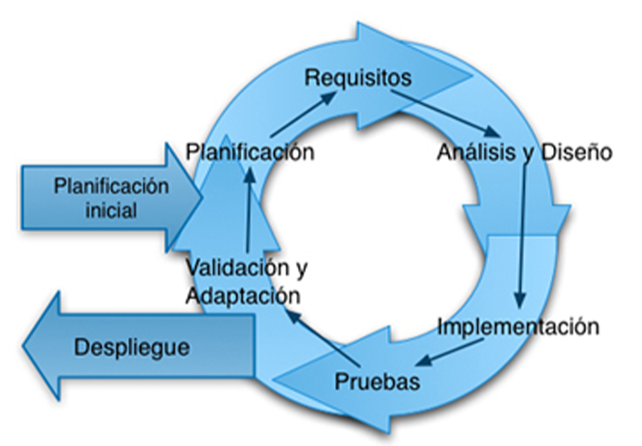
\includegraphics[width=0.7\textwidth]{img/Iterativoincremental.png}
    \caption{Ciclo de vida del desarrollo software iterativo \cite{Pradel2013} }
    \label{fig:iterativoincremental}
\end{figure}
Cada iteración durará entre 1 y 6 semanas, siendo ideal mantener una duración uniforme entre las distintas iteraciones. Al finalizar cada iteración, se tendrán en cuenta los resultados obtenidos para adaptar la planificación, requisitos y demás fases de las iteraciones posteriores.\\
A lo largo de este proyecto se realizaron 5 iteraciones de desarrollo software (partiendo del desarrollo software en el TFG \cite{Martos2024}), resultando la duración de las mismas algo dispar debido a complicaciones técnicas que se produjeron en algunas de ellas:
\begin{itemize}
    \item Primera iteración (semanas 1-2): generación de gráficas a partir de las actividades almacenadas en la base de datos. Generación y descarga automática de informe médico incluyendo dicha información de actividades y de forma opcional las gráficas. Para realizar pruebas durante esta iteración se utilizó el prototipo hardware construido en el TFG \cite{Martos2024}.
    \item Segunda iteración (Semanas 3-4): Personalización del tiempo de reposo que el script Arduino detecta como congelación de la marcha mediante la realización de una sencilla prueba. Para probar los resultados de esta iteración también se utilizó el prototipo hardware construido en el TFG \cite{Martos2024}.
    \item Tercera iteración (Semenas 5-10): Implementación de un diario de fluctuaciones motoras. Mejora de las funcionalidades anteriores. Se realizaron las pruebas de funcionamiento de dichas mejoras utilizando Protoboards de Arduino como montaje provisional del nuevo hardware.
    \item Cuarta iteración (Semanas 11-13): Almacenamiento de datos del diario de fluctuaciones en la base de datos, registro de la hora y fecha de las actividades realizadas. Las pruebas de esta iteración pudieron realizarse en un modelo definitivo del nuevo hardware.
    \item Quinta iteración (Semanas 14-15): Gestión de los datos de actividades registradas y diarios para la realización de gráficas relevantes sobre los mismos. Pruebas finales de funcionamiento.
\end{itemize}
\subsection{Herramientas software}
\begin{itemize}
    \item XAMPP: Herramienta que permite la instalación de un servidor web en el dispositivo. En concreto se han utilizado los componentes del servidor web Apache y MySQL. Ha resultado útil para continuar el desarrollo de la aplicación web de forma local.
    \begin{itemize}
    \item MySQL: Este componente de XAMPP permite la gestión de bases de datos de forma local. Se ha utilizado para generar tablas para el almacenamiento de datos del diario de tomas y de fluctuaciones motoras.
    \end{itemize}
    \item Visual Studio Code: Aplicación para el desarrollo de código que permite la utilización de diferentes lenguajes de programación dentro de la misma. Se ha utilizado para generar archivos .php, en los cuales se incluyó código HTML y Javascript, así como para la edición de archivos .js que manejan la comunicación bidireccional entre la aplicación web y el código de Arduino.
    \item IDE Arduino: Entorno de desarrollo software para la escritura, compilación y carga de código en placas de Arduino. Se utilizó para modificar el script Arduino, incluyendo la personalización de bloqueos, el manejo del módulo láser...
    \item Autodesk Sketchbook: Software utilizado para el desarrollo de planos del hardware a desarrollar.
    \item Microsoft Visio: Software de diagramación utilizado para ilustrar las conexiones entre los componentes hardware y la placa Arduino Uno.
    \item Microsoft Excel: Software de hojas de cálculo que ha sido utilizado para la realización de los diagramas de Gantt que ilustran la planificaicón del proyecto.
    \item Versión 2 de ChatGPT: IA de conversación creada por OpenAI que ha sido utilizada en ocasiones como apoyo durante el desarrollo de software.
    \item Lucidchart: Software de creación de diagramas online utilizado para la creación de diagramas incluidos en los Anexos.
    \item Balsamiq Wireframes: Software de creación de prototipos de interfaces y wireframes, que ha sido utilizada para la creación de los wireframes de la página web incluidos en los Anexos.
    \item Visual paradigm: Software de creación online de diagramas UML, utilizado para la creación del diagrama de despliegue incluido en los anexos.
    \item Tinkercad: software online que permite crear diseños 3D así como crear y simular el funcionamiento de circuitos electrónicos. Se utilizó para ilustrar la conexión de algunos componentes hardware a la placa Arduino en los anexos.
\end{itemize}
\subsubsection{Lenguajes de programación}
\begin{itemize}
    \item PHP: Este lenguaje de programación permite el desarrollo backend en aplicaciones web. Se utilizó mayoritariamente como enlace entre los formularios mostrados en pantalla y la base de datos, recogiendo al enviarse el formulario los datos insertados e insertándolos en filas de la tabla correspondiente en la base de datos. Adicionalmente se utilizó de forma complementaria en los documentos destinados al desarrollo frontend para realizar funciones complejas no realizables mediante HTML.
    \item Javascript: Este lenguaje permite la creación de contenido dinámico e interactivo en aplicaciones web. Se utilizó principalmente para otorgar dinamismo a formularios web en el frontend.
    \item HTML: Este lenguaje permite la creación de contenido estático en aplicaciones web. Se utilizó principalmente en el desarrollo de formularios para el registro diario de fluctuaciones y tomas, complementándolo con el uso de CSS para manejar el estilo del contenido.
    \item Python: Este lenguaje de programación se utilizó para generación de pdfs y gráficas a partir de las actividades registradas.
    \item Arduino C/C++: El lenguaje de programación utilizado en IDE Arduino, constituye una variante simplificada de los lenguajes de programación C/C++.
\end{itemize}
\subsubsection{Bibliotecas utilizadas en los distintos lenguajes de programación}
\begin{enumerate}
    \item \textbf {Bibliotecas de python utilizadas para la generación de PDFs}
        \begin{itemize}
            \item 'Reportlab': Biblioteca para la generación de documentos PDF. En los archivos 'pdf.py' y 'pdf2.py' se utilizaron los siguientes submódulos o clases de esta bibioteca:
            \begin{itemize}
                \item 'reportlab.lib.pagesizes.letter'
                \item 'reportlab.platypus.SimpleDocTemplate'
                \item 'reportlab.platypus.Paragraph'
                \item 'reportlab.platypus.Spacer'
                \item 'reportlab.platypus.Table'
                \item 'reportlab.lib.styles.getSampleStyleSheet'
                \item 'reportlab.lib.colors'
                \item 'reportlab.platypus.Image'
            \end{itemize}
            \item 'Urllib': Biblioteca que permite trabajar con URLs. En concreto, se usó la función 'urllib.request.urlretrieve', que permite descargar archivos desde una URL y guardarlos correctamente.
            \item 'os': Biblioteca para interactuar con el sistema operativo.
            \item 'json': Biblioteca que permite trabajar con datos JSON.
            \item 'mysql.connector': Biblioteca para la conexión e interacción con bases de datos MySQL.
        \end{itemize}
    \item \textbf {Bibliotecas/funciones de python utilizadas para la generación de gráficas}
            \begin{itemize}
                \item 'os': Biblioteca para interactuar con el sistema operativo.
                \item 'sys': Funciones y variables que interactúan con el intérprete de python.
                \item 'json': Biblioteca que permite trabajar con datos JSON.
                \item 'matplotlib.pyplot': herramienta para la creación de gráficas.
                \item 'Ipython.display': funciones que permiten mostrar contenidos multimedia en notebooks de python.
                \item 'mysql': Paquete que permite interactuar con bases de datos MySQL. Dentro del mismo, se utilizan las funciones 'mysql.connector' para conectar y ejecutar consultas con bases de datos MySQL.
                \item 'pandas': Biblioteca para la manipulación y análisis de datos de tablas.
                \item 'sqlalchemy': Biblioteca que permite conectarse con bases de datos relacionales con la función 'create engine', que crea un motor o representación abstracta de la base de datos a la cual se conecta con sqlalchemy.
            \end{itemize}
    \item \textbf {Bibliotecas/funciones de otros lenguajes de programación }
Como bibliotecas y funciones de los lenguajes de programación PHP y Arduino se utilizaron principalmente los recursos descritos en el TFG \cite{Martos2024}. Se utilizó también la biblioteca de Arduino 'RTClib.h' durante los intentos de inclusión del módulo RTC en el hardware. Sin embargo, como se describe en el apartado 'Conclusiones', esta biblioteca no se utiliza en el prototipo presentado debido a la decisión de no incluir dicho módulo.
\end{enumerate}



\subsection{Herramientas hardware}
Se reconstruyó el hardware presentado en el TFG \cite{Martos2024}, incluyendo también un módulo láser y rediseñando el prototipo para insertarlo en un cinturón y tobillera, como se muestra en la figura \ref{fig:esquemahardware}. En esta imagen podemos observar una primera banda, en la que se representan los componentes adheridos a la zona exterior del cinturón, una segunda banda con los componentes adjeridos a la zona interior del cinturón y el sensor MPU-6050, insertado en la tobillera y comunicado con el cinturón mediante un cable multihilo. 
El circuito de conexión de los componentes hardware a la placa Arduino se realizó mediante el Arduino proto shield, siguiendo el esquema mostrado en la figura \ref{fig:esquemacircuito}. Adicionalmente a las conexiones representadas en esta figura, se alimentó la placa Arduino mediante una batería. Esta alimentación se controlaba mediante el interruptor ON/OFF (la conexión de estos componentes puede observarse también en la figura \ref{fig:esquemahardware}).
\begin{figure}[h]
    \centering
    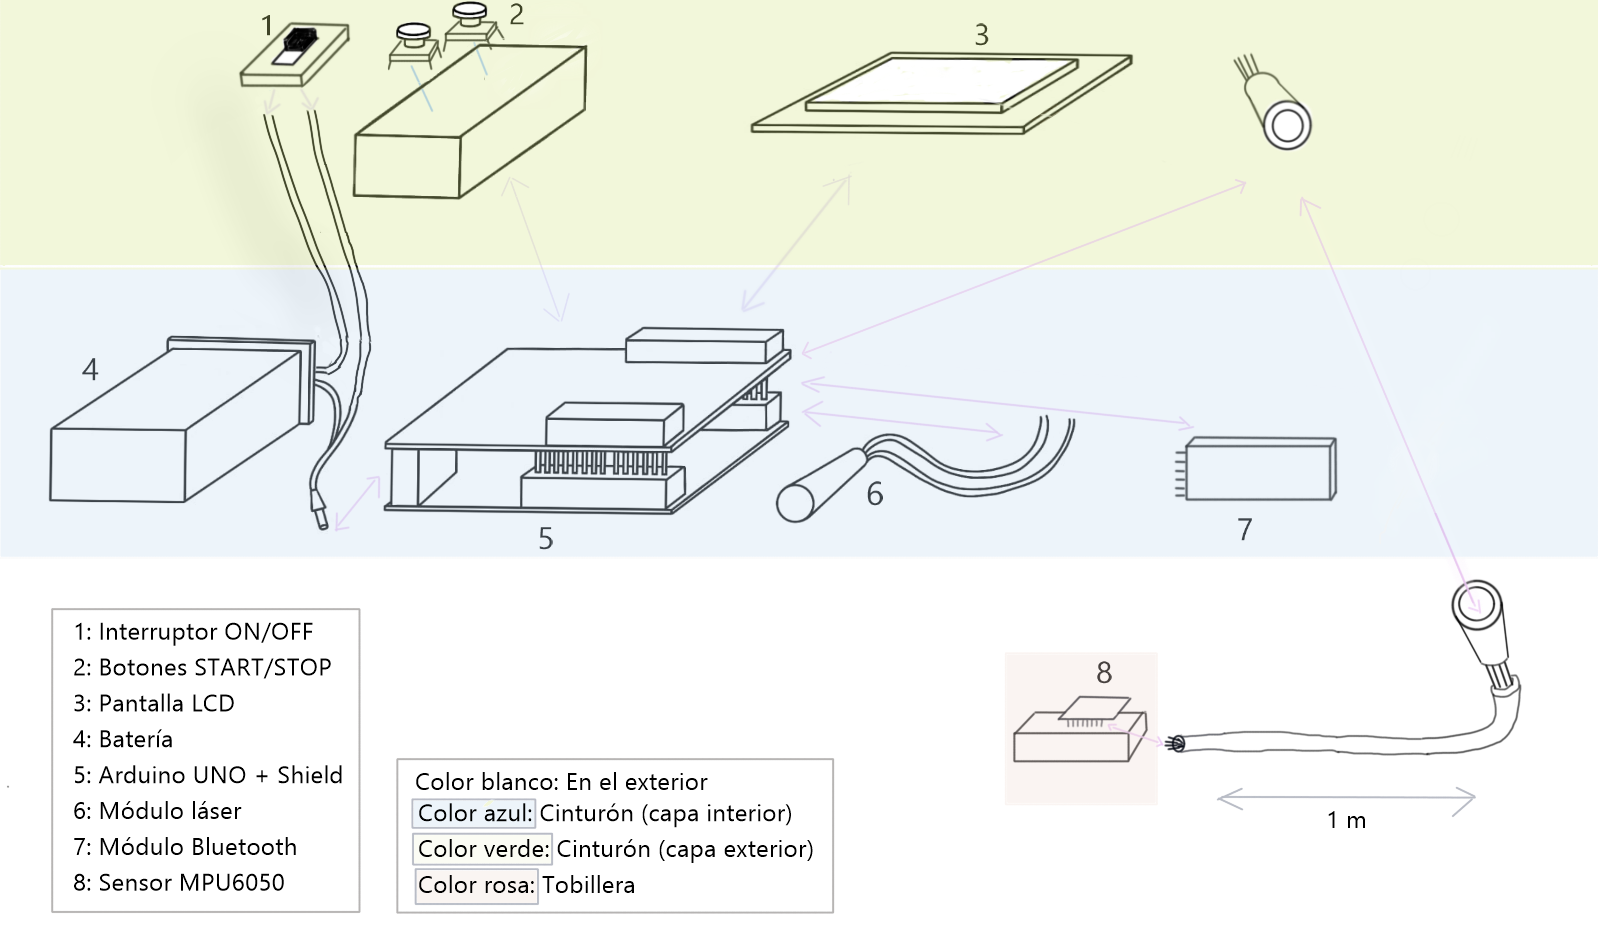
\includegraphics[width=1\textwidth]{img/esquemahardware.png}
    \caption{Esquema de la colocación de elementos hardware en el prototipo}
    \label{fig:esquemahardware}
\end{figure}
\begin{sidewaysfigure}[h]
    \centering
    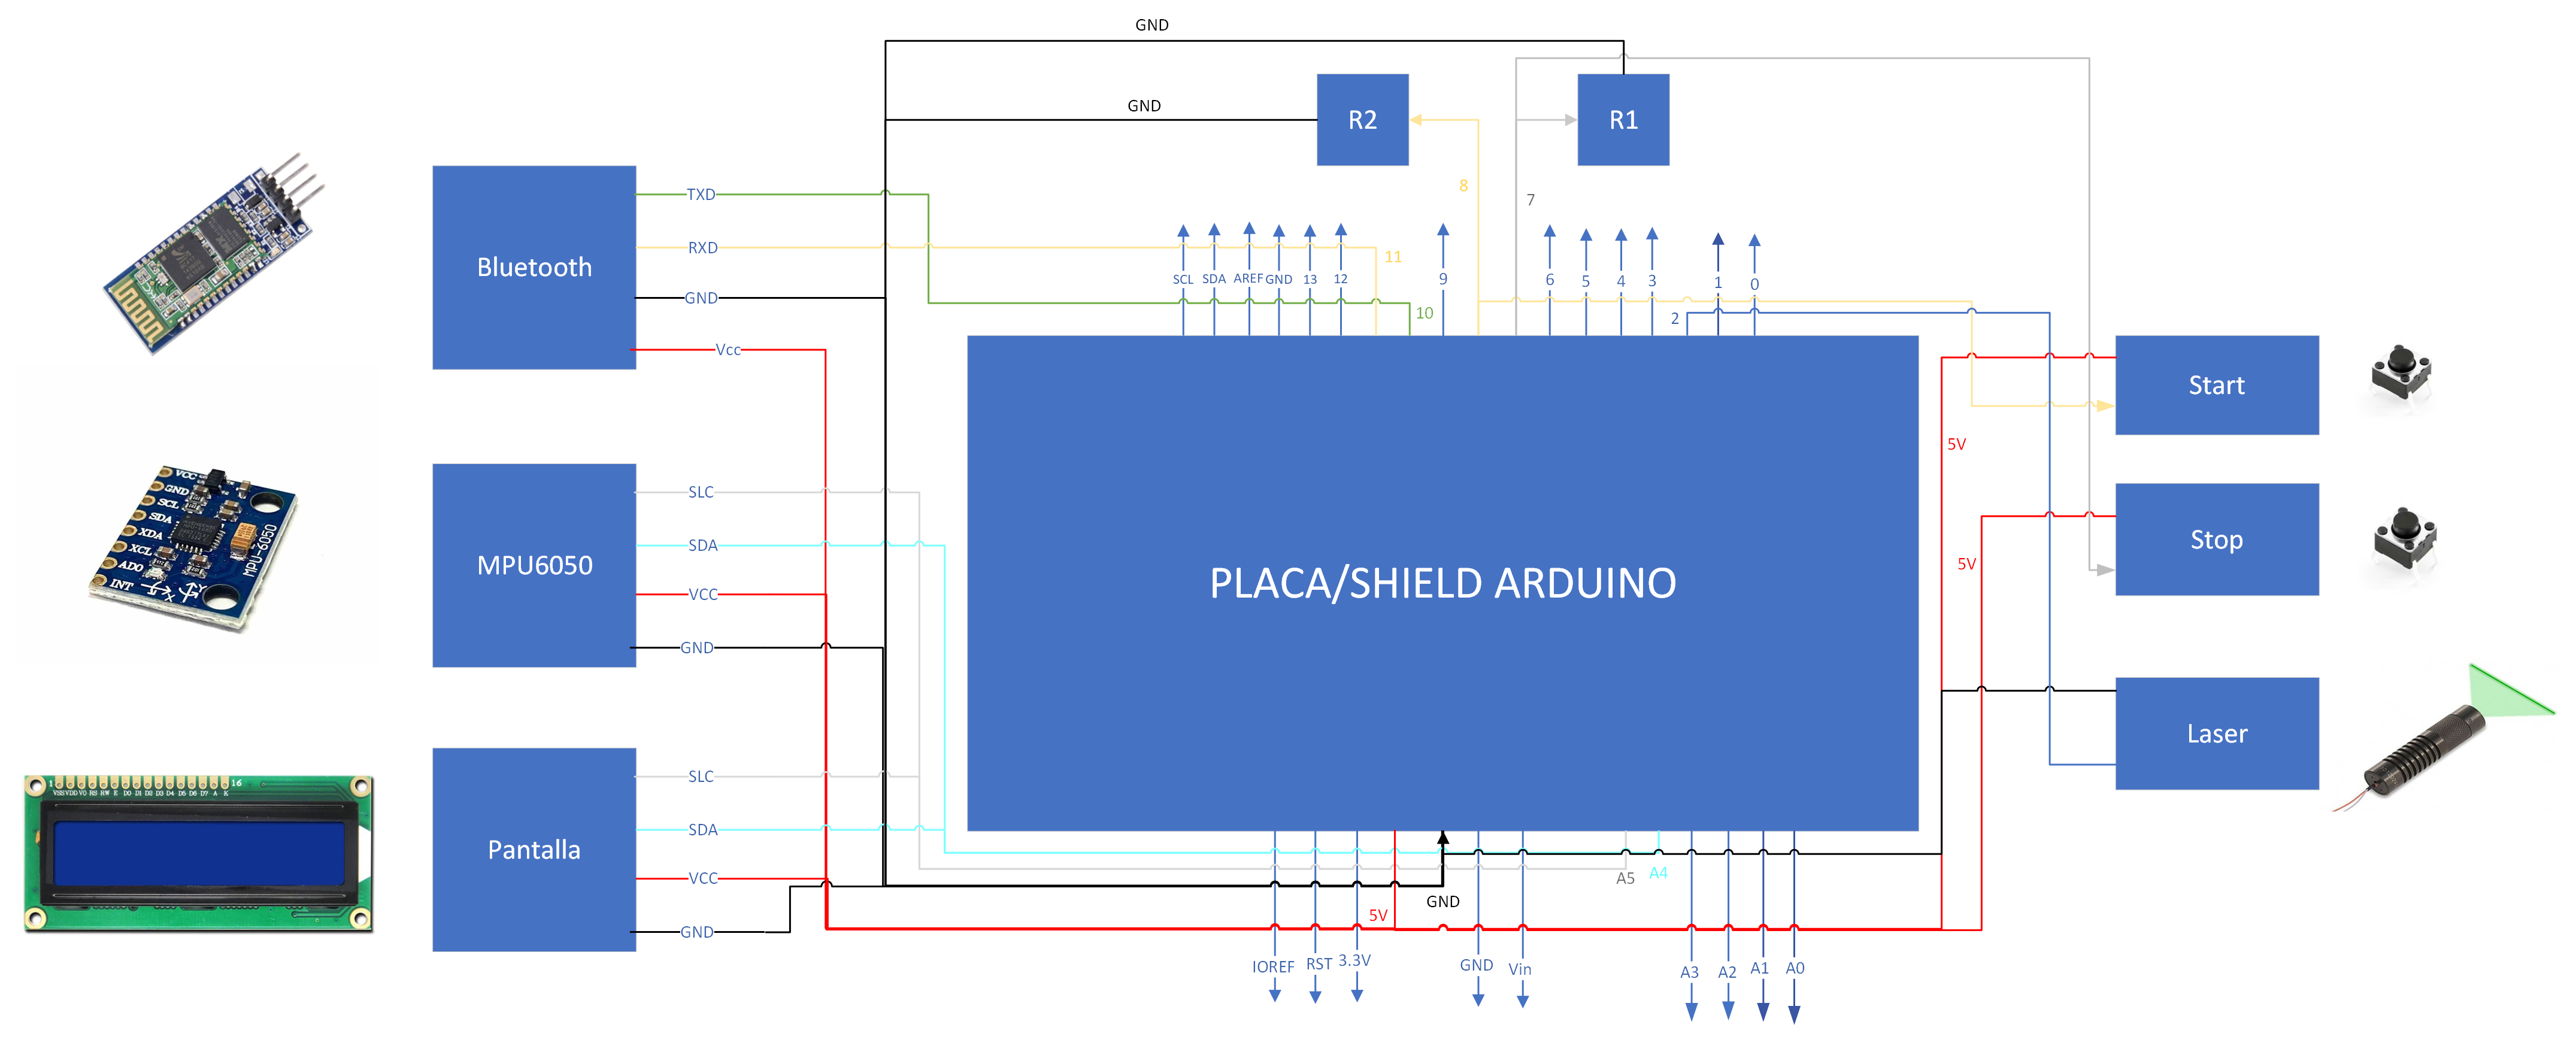
\includegraphics[width=1\textwidth]{img/circuito.png}
    \caption{Esquema del circuito formado por la placa Arduino UNO y los componentes conectados a la misma}
    \label{fig:esquemacircuito}
\end{sidewaysfigure}
Los componentes hardware utilizados para el diseño de este prototipo fueron:
\begin{itemize}
\item Microcontrolador Arduino UNO R3: Microcontrolador Arduino basado en ATmega328P, que consta de 14 pines digitales, 6 pines analógicos, conexión USB y toma de corriente.\ref{fig:unor3}
\begin{figure}
    \centering
    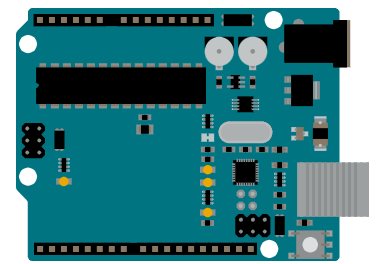
\includegraphics[width=0.5\textwidth]{img/unor3.png}
    \caption{Arduino UNO R3}
    \label{fig:unor3}
\end{figure}
\item Fuente de alimentación 9V
\item Interruptor ON/OFF
\item Pantalla LCD 16x2 con módulo LCD I2C \ref{fig:pantalla}: Esta pantalla de permite la visualización simultánea de 2x16 caracteres. El módulo LCD nos permite conectar con la pantalla empleando tan sólo 4 pines, haciendo más sencilla la integración en el circuito. \begin{figure}[h]
    \centering
    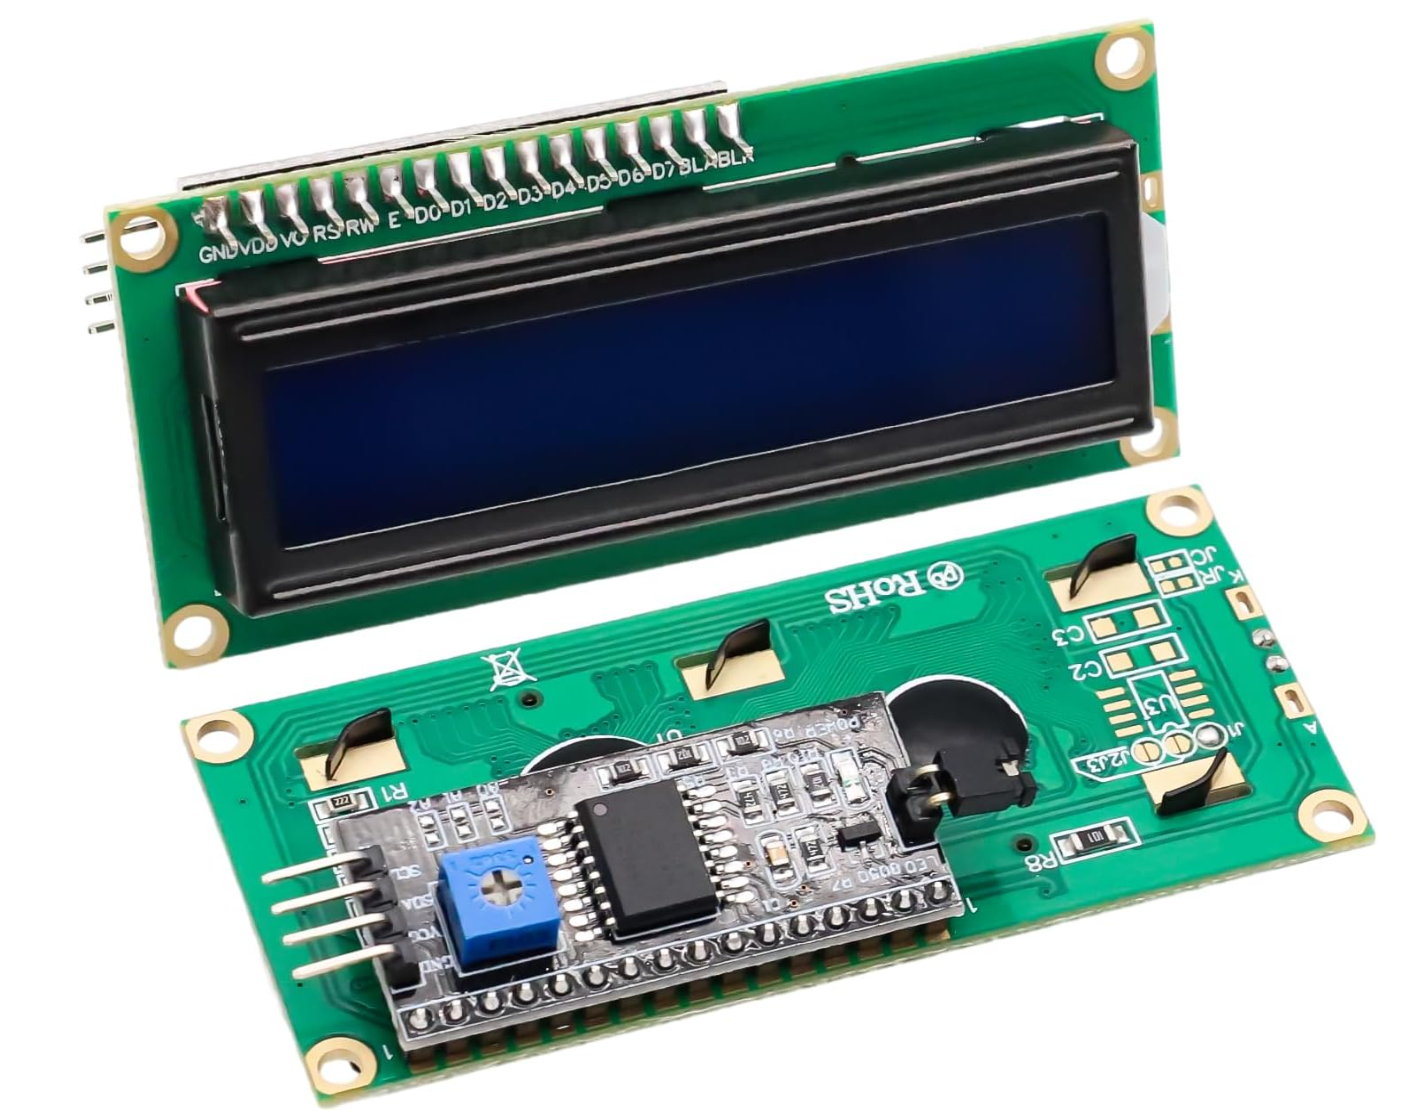
\includegraphics[width=0.8\textwidth]{img/pantalla.png}
    \caption{Pantalla LCD 16x2 con módulo LCD I2C \cite{ARCELI_LCD_Module}}
    \label{fig:pantalla}
\end{figure}
\item 2 pulsadores: Se utilizaron 2 pulsadores como botones de start/stop del dispositivo.
\item Módulo láser \ref{fig:laser}: Se incluyó un módulo láser que proyecta una línea recta en el suelo como respuesta a la detección de un congelamiento de la marcha.
\begin{figure}
    \centering
    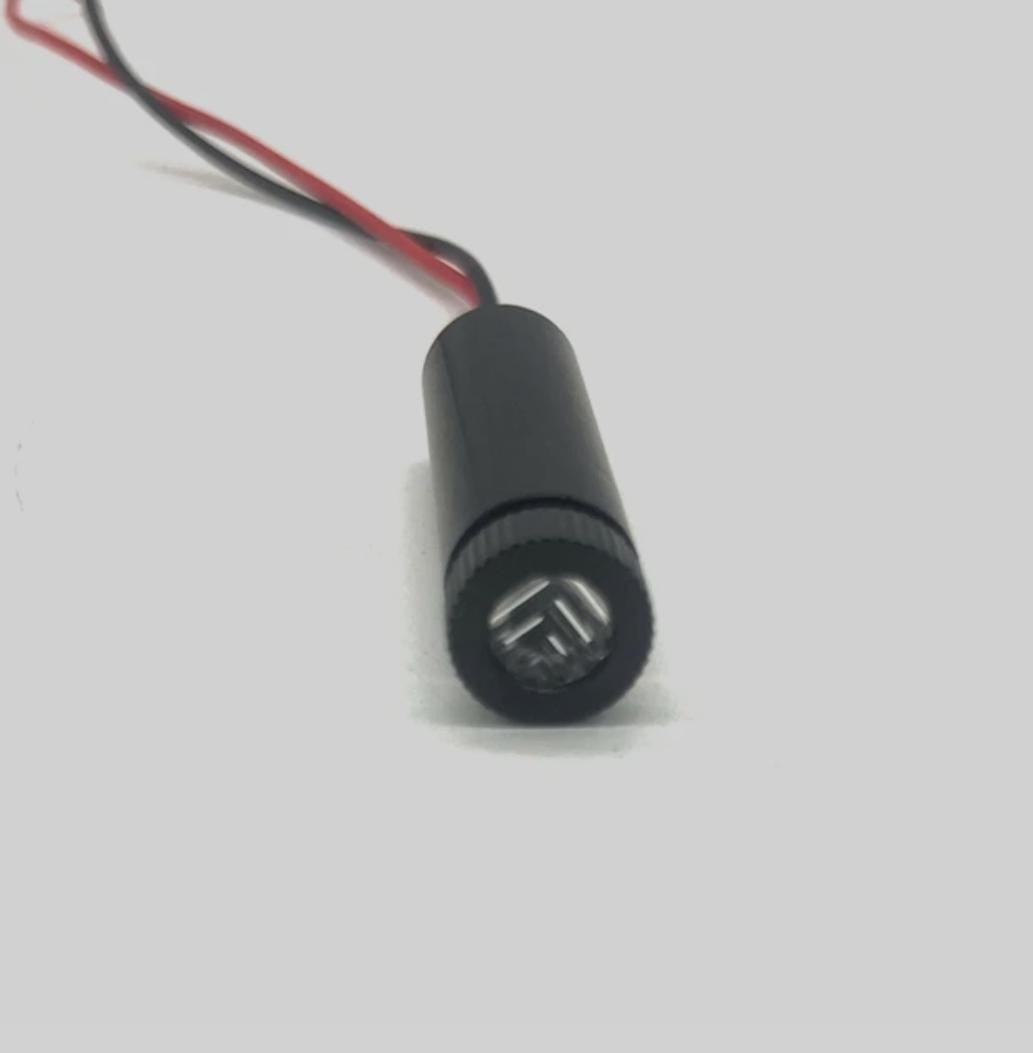
\includegraphics[width=0.5\textwidth]{img/laser.jpg}
    \caption{Módulo láser. \cite{LaserModule}}
    \label{fig:laser}
\end{figure}
\item Módulo bluetooth HC-05 \ref{fig:bluetooth}: Se utilizó este módulo de comunicación bluetooth serial para permitir la conexión inalámbrica entre el dispositivo y la aplicación web.
\begin{figure}
    \centering
    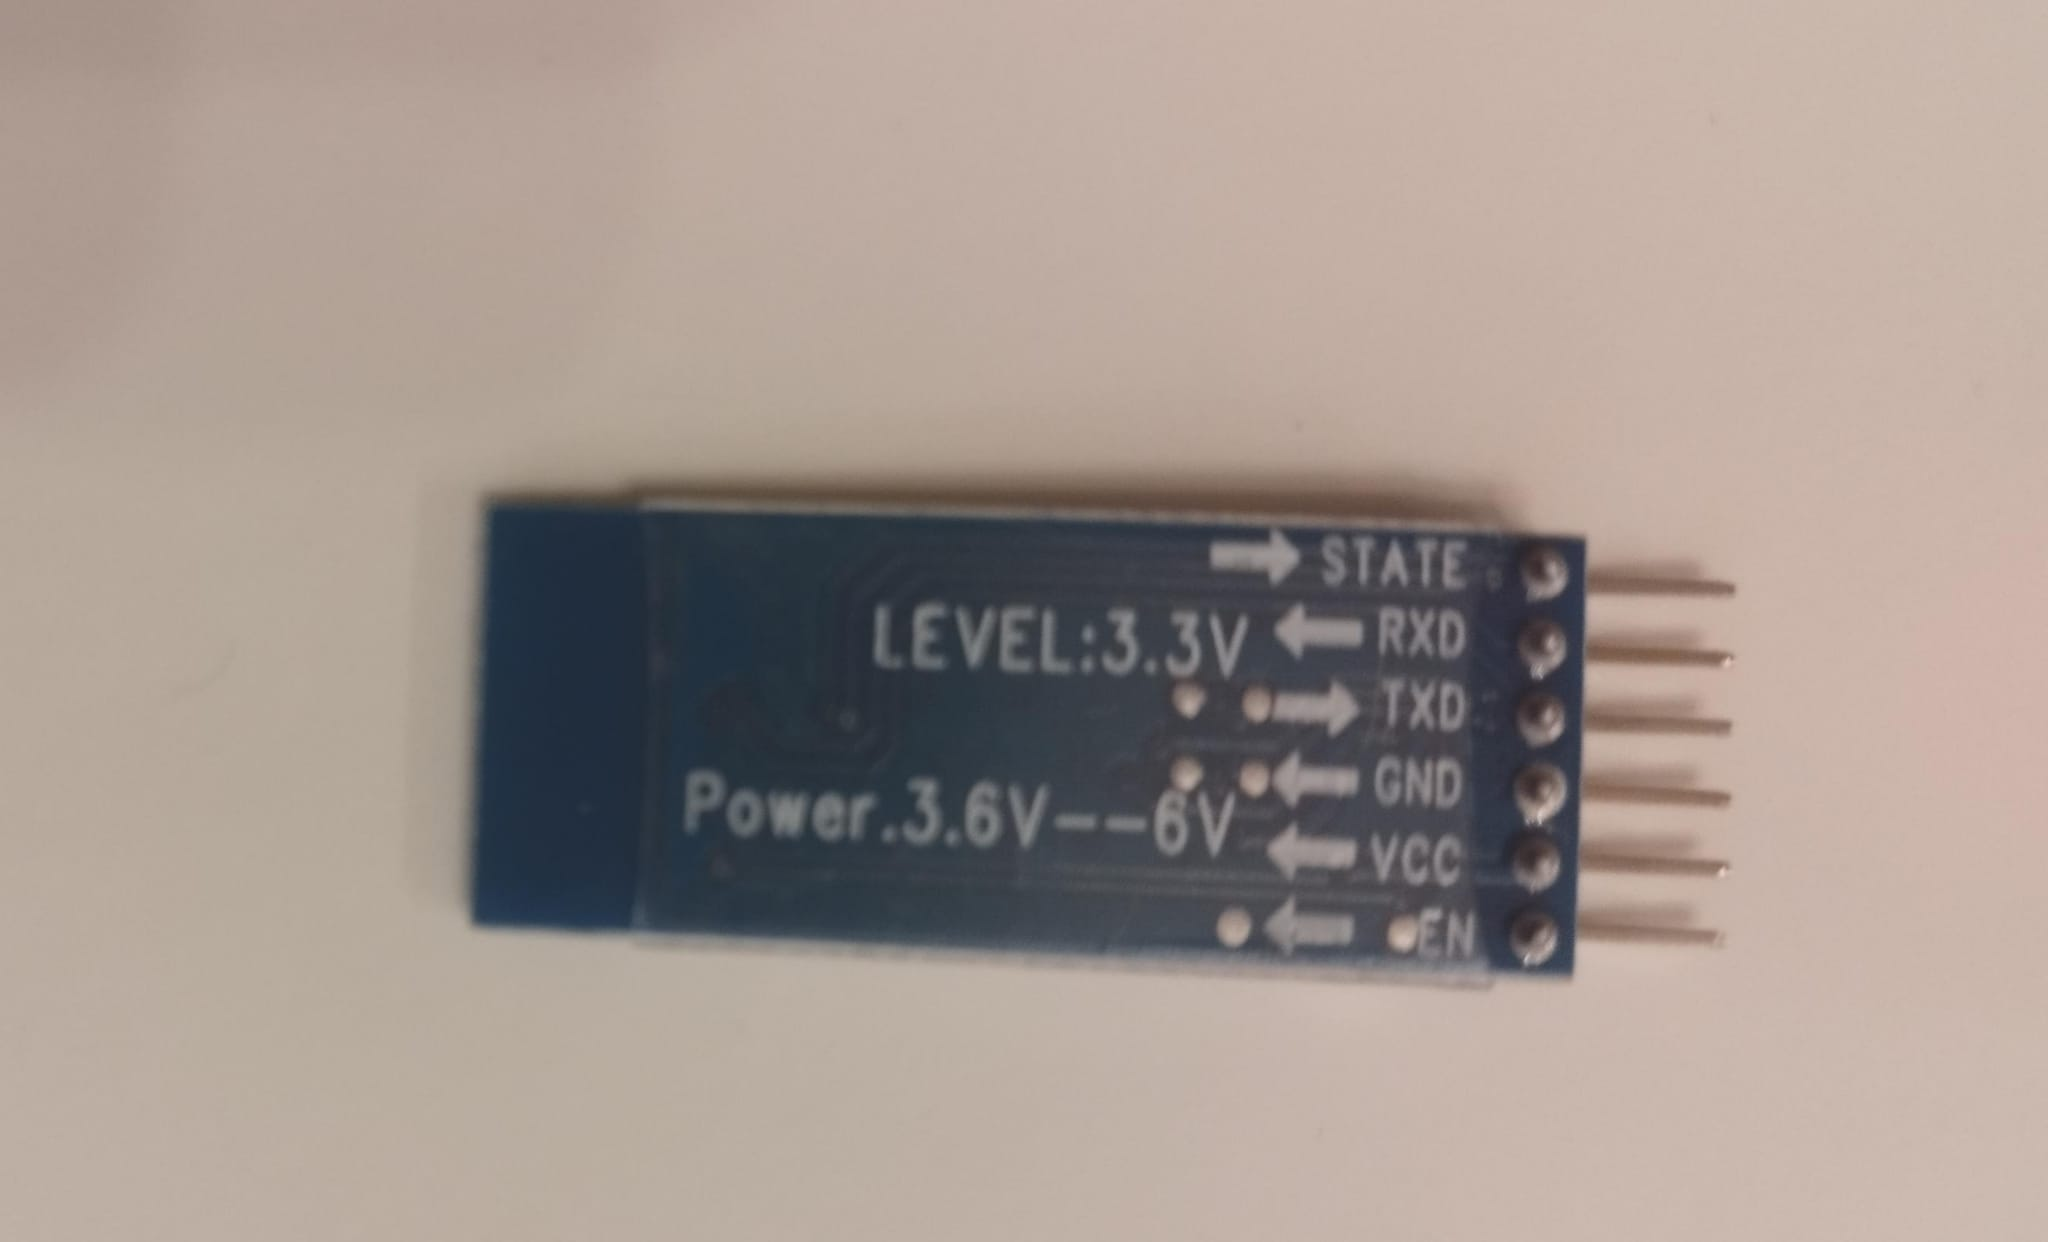
\includegraphics[width=0.5\textwidth]{img/bluetooth.jpg}
    \caption{Módulo bluetooth HC-05}
    \label{fig:bluetooth}
\end{figure}
\item Cable multihilo: como conexión entre el cinturón y la tobillera se utilizó un cable multihilo
\item Sensor MPU-6050 \ref{fig:mpu}: Se utilizó este sensor de movimiento y giroscopio de seis ejes para recoger los datos del acelerómetro y giroscopio relacionados con la marcha del paciente.

\begin{figure}
    \centering
    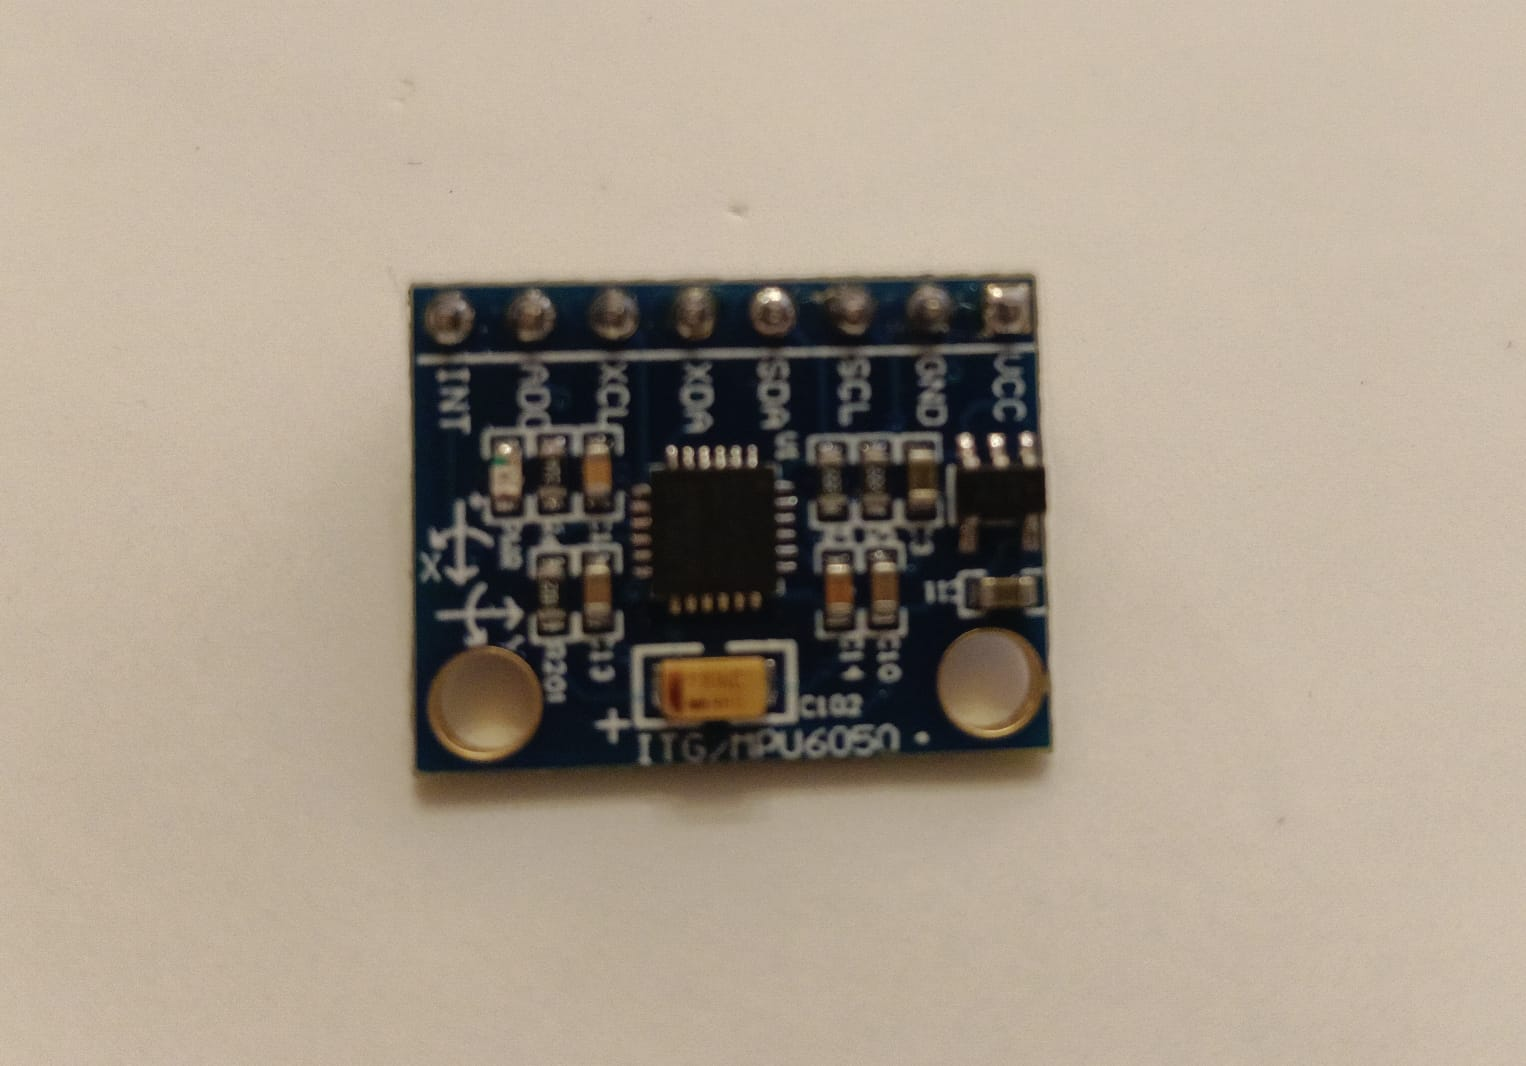
\includegraphics[width=0.5\textwidth]{img/mpu6050.jpg}
    \caption{Sensor MPU-6050. Fuente propia.}
    \label{fig:mpu}
\end{figure}
\end{itemize}
%Esta parte de la memoria tiene como objetivo presentar las técnicas metodológicas y las herramientas de desarrollo que se han utilizado para llevar a cabo el proyecto. Si se han estudiado diferentes alternativas de metodologías, herramientas, bibliotecas se puede hacer un resumen de los aspectos más destacados de cada alternativa, incluyendo comparativas entre las distintas opciones y una justificación de las elecciones realizadas. 
%No se pretende que este apartado se convierta en un capítulo de un libro dedicado a cada una de las alternativas, sino comentar los aspectos más destacados de cada opción, con un repaso somero a los fundamentos esenciales y referencias bibliográficas para que el lector pueda ampliar su conocimiento sobre el tema.

 